% vim:syntax=tex

In this section we describe the design of a study in which we compare topic models trained on changesets to those trained on snapshots.
We describe the case study using the Goal-Question-Metric approach~\cite{Basili-etal:94}.
The data and source code for the case study is available in this paper's online
appendix\footnote{\textbf{REVIEWER URL ONLY:} \url{http://christop.club/x/cfl/}}.

\subsection{Definition and Context}

% TODO
Our \textit{goal} is to evaluate the effective nature of topic models built
from changesets.
The \textit{quality focus} of the study is on informing development
decisions and policy changes that could lead to software with fewer
defects.
The \textit{perspective} of the study is of a researcher, developer, or
project manager who wishes to gain understanding of the concepts or
features implemented in the source code.
The \textit{context} of the study spans the version histories of 14
open source systems.

Toward the achievement of our goal, we pose the following research questions:
\begin{description}[font=\itshape\mdseries,leftmargin=10mm,style=sameline]
% TODO
    \item[RQ1] Is a changeset-based FLT on par with a snapshot-based FLT?
    \item[RQ2] Are FLTs accurately evaluated in life-like evaluation scenarios?
\end{description}

At a high level, our goal is to determine the feasibility in using changesets
to train topic models for feature location.

In the remainder of this section we introduce the subjects of our study,
describe the setting of our study, and report our data collection and analysis procedures.

%%%%%%%%%%%%%%%%%%%%%%%%%%%%%%%%%%%%%%%%%%%%%%%%%%%%%%%%%%%%%%%%%%%%%%%%

\subsection{Subject software systems}

All of our subject software systems come from two publicly-available datasets.
The first is a dataset of six software systems by Dit et al.~\cite{Dit-etal:2013} and contains method-level goldsets.
This dataset was automatically extracted from changesets that relate to the queries (issue reports).
The second is a dataset of 14 software systems by Moreno et al.~\cite{Moreno-etal:2014} and contains class-level goldsets.
This dataset was automatically extracted from patches attached to issue reports.
The six software systems in the first dataset also appear in the second,
supplying us with both class- and method-level goldsets for the queries.

\begin{table}[t]
\renewcommand{\arraystretch}{1.3}
\footnotesize
\centering
\caption{Subject Systems and Goldset Sizes}
\begin{tabular}{lrrr}
    \toprule
    Subject System     & Features & Classes & Methods \\
    \midrule
    ArgoUML v0.22      & 91       & 287     & 701     \\
    ArgoUML v0.24      & 52       & 154     & 357     \\
    ArgoUML v0.26.2    & 209      & 706     & 1560    \\
    BookKeeper v4.1.0  & 40       & 152     &         \\
    Derby v10.7.1.1    & 32       & 55      &         \\
    Derby v10.9.1.0    & 95       & 410     &         \\
    Hibernate v3.5.0b2 & 20       & 53      &         \\
    Jabref v2.6        & 39       & 131     & 280     \\
    jEdit v4.3         & 150      & 361     & 748     \\
    Lucene v4.0        & 35       & 103     &         \\
    Mahout v0.8        & 30       & 159     &         \\
    muCommander v0.8.5 & 92       & 303     & 717     \\
    OpenJPA v2.0.1     & 35       & 82      &         \\
    OpenJPA v2.2.0     & 18       & 53      &         \\
    Pig v0.8.0         & 85       & 442     &         \\
    Pig v0.11.1        & 48       & 129     &         \\
    Solr v4.4.0        & 55       & 189     &         \\
    Tika v1.3          & 18       & 34      &         \\
    ZooKeeper v3.4.5   & 80       & 285     &         \\
    \midrule
    Total              & 1224     & 4088    & 4363    \\
    \bottomrule
\end{tabular}
\label{table:subjects}
\end{table}

ArgoUML is a UML CASE tool that supports standard UML diagrams\footnote{\url{http://argouml.tigris.org/}}.
BookKeeper is a distributed logging service\footnote{\url{http://zookeeper.apache.org/bookkeeper/}}.
Derby is a relational database management system\footnote{\url{http://db.apache.org/derby/}}.
Eclipse is an IDE for development in various programming languages\footnote{\url{https://www.eclipse.org/}}.
Hibernate is a object and relational mapping framework\footnote{\url{http://hibernate.org/}}.
JEdit is a Java text editor\footnote{\url{http://www.jedit.org/}}.
JabRef is a tool for managing bibliographical reference data\footnote{\url{http://jabref.sourceforge.net/}}.
Lucene is an information retrieval library\footnote{\url{http://lucene.apache.org/core/}}.
Mahout is a tool for scalable machine learning\footnote{\url{https://mahout.apache.org/}}.
MuCommander is a cross-platform file manager\footnote{\url{http://www.mucommander.com/}}.
OpenJPA is object relational mapping tool\footnote{\url{http://openjpa.apache.org/}}.
Pig is a platform for analyzing large datasets consisting of high-level language\footnote{\url{http://pig.apache.org/}}.
Solr is an enterprised search platform\footnote{\url{http://lucene.apache.org/solr/}}.
Tika is a toolkit for extracting metadata and text from various types of files\footnote{\url{http://tika.apache.org/}}.
ZooKeeper is a tool that works as a coordination service to help build distributed applications\footnote{\url{http://zookeeper.apache.org/bookkeeper/}}.


%%%%%%%%%%%%%%%%%%%%%%%%%%%%%%%%%%%%%%%%%%%%%%%%%%%%%%%%%%%%%%%%%%%%%%%%

\subsection{Methodology}
\label{sec:methodology}

For snapshots, the process is straightforward and corresponds to
Figure~\ref{fig:snapshot}.  First, we build a model in batch mode from the
snapshot corpus.  That is, the model can see all documents in the corpus at
once.  Then, we infer an index of topic distributions from the snapshot corpus.
For each query in the dataset, we infer the query's topic distribution and rank
each entity in the index with pairwise comparisons.

\begin{comment}
\begin{enumerate}
    \item Build model from the snapshot corpus in batch mode
    \item Infer a $\theta_{Snapshot}$ from the snapshot corpus
    \item Infer a $\theta_{Queries}$ from the query corpus
    \item Classify, or rank, the results from both $\theta$s
\end{enumerate}
\end{comment}


In terms of changesets, the process varies slightly from a snapshot approach, as
shown in Figure~\ref{fig:changeset}.  First, we build a model in batch mode
from the changeset corpus.  Second, we infer an index of topic distributions
from the snapshot corpus and a topic distribution of the query.  Note that we
\emph{do not} infer topic distributions from the changeset corpus on which the
model was built.  Finally, for each query in the dataset, we infer the query's
topic distribution and rank each entity in the snapshot index with pairwise
comparisons.

\begin{comment}
\begin{enumerate}
    \item Build model from the changeset corpus in batch mode
    \item \emph{Do not} infer a $\theta_{Changesets}$
    \item Infer a $\theta_{Snapshot}$ from the snapshot corpus
    \item Infer a  $\theta_{Queries}$ from the query corpus
    \item Classify, or rank, the results from both $\theta$s
\end{enumerate}
\end{comment}


For the historical simulation, we can take a slightly different approach.  We
first determine which changesets relate to each query (or issue) and partition
mini-batches out of the changesets.  We then proceed by initializing a model in
online mode.  Using each mini-batch, or partition, we update the model.  Then,
we infer an index of topic distributions from the snapshot corpus at that
commit.  We also obtain a topic distribution for each query related to the
changeset of interest.  For each query in the dataset related to the changeset,
we infer the query's topic distribution and rank each entity in the snapshot
index with pairwise comparisons. Finally, we continue by updating the model with
the next mini-batch.

\begin{comment}
\begin{enumerate}
    \item Initialize a model in online mode
    \item Determine which changesets relate to an issue and partition mini-batches out of the changesets
    \item For each mini-batch:
        \begin{enumerate}
            \item Update the model with mini-batch
            \item Update $\theta_{Snapshot}$ with the new inference of the source code document affected by this changeset
            \item Infer a $\theta_{Query}$ of the query related to the changeset we stopped at
            \item Classify, or rank, the results from both $\theta$s
        \end{enumerate}
\end{enumerate}
\end{comment}

Since the Dit et al. dataset was extracted from the commit that implemented the
change, our partitioning is inclusive of that commit.  That is, we update the
model with the linked commit and infer the snapshot index from that commit.
This allows our evaluation to capture any entities added to address the issue
report, as well as changed entities, but does not capture any entities that were
removed by the change.



%%%%%%%%%%%%%%%%%%%%%%%%%%%%%%%%%%%%%%%%%%%%%%%%%%%%%%%%%%%%%%%%%%%%%%%%

\subsection{Setting}

Our document extraction process is shown on the left side of Figure~\ref{fig:changeset}
We implemented our document extractor in Python v2.7
using the Dulwich library\footnote{\url{http://www.samba.org/~jelmer/dulwich/}}
for interacting with the source code repository and
Taser for parsing source code.
We extract documents from both a snapshot of the repository at a tagged
snapshot and each commit reachable from that tag's commit.
The same preprocessing steps are employed on all documents extracted.

For our document extraction from a snapshot, we first parse each Java file using our tool, Taser.
Taser is a text extractor implemented in Java using an open source Java 1.5 grammar and ANTLR v3.
The tool extracts documents from the chosen source code entity type,
either methods or classes, and treats inner entities to be distinct from the outer entity.
We consider interfaces, enumerations, and annotation types to also be a class.
The text of inner an entity (e.g., a method inside an anonymous class)
is only attributed to that entity, and not the containing one.
Comments, literals, and identifiers within a entity are considered as text of the entity.
Block comments immediately preceding an entity are also included in this text.

To extract text from the changesets, we look at
the \texttt{git diff} between two commits.
In our changeset text extractor, we extract all text related to the
change, e.g., context, removed, and added lines; metadata lines are ignored.
Note that we do not consider where the text originates from,
only that it is text changed by the commit.%\footnote{
%The Apache Lucene and Solr projects were merged into a single, new repository
%during their development.
%We only use changes that affect each project's subdirectory in the merged repository,
%and also include all changes from the two pre-merge repositories in each project's respective corpus.
%}

After extracting tokens, we split the tokens based on camel case,
underscores, and non-letters.
We only keep the split tokens; original tokens are discarded.
We normalize to lower case before filtering non-letters, English stop words~\cite{StopWords}, Java keywords, and words shorter than three characters long.
We do not stem words.

We implemented our modeling using the Python library Gensim~\cite{Gensim},
version 0.10.3. We use the same configurations on each subject system.  We do
not try to adjust parameters between the different models to attempt to find
a better, or best, solution; rather, we leave them the same to reduce
confounding variables.  We do realize that this may lead to topic models that
are not best-suited for feature location on a particular subject system.
However, this gives us confidence that the measurements collected are fair, and
that the results are not influenced by selective parameter tweaking.  Again, our
goal is to show the performance of the changeset-based FLT against
snapshot-based FLT under the same conditions.

Gensim's LDA implementation is based on an online LDA by Hoffman et
al.~\cite{Hoffman-etal:2010} and uses variational inference instead of
a Collapsed Gibbs Sampler.  Unlike Gibbs sampling, in order to ensure that the
model converges for each document, we allow LDA to see each mini-batch $5$ times
by setting Gensim's initialization parameter \texttt{passes} to this value and
allowing the inference step $1000$ iterations over a document.  We set the
following LDA parameters for all 14 systems: $500$ topics ($K$), a symmetric
$\alpha=1/K$, and a symmetric $\eta=1/K$.  These are default values for
$\alpha$ and $\eta$ in Gensim.

For the historical simulation, we found it beneficial to consider two other
parameters: $\kappa$ and $\tau_0$.  As noted in Hoffman et
al.~\cite{Hoffman-etal:2010}, it is beneficial to adjust $\kappa$ and $\tau_0$
to higher values for smaller mini-batches.  These two parameters control how
much influence a new mini-batch has on the model when training.  We follow the
recommenations in Hoffman et al.\, chosing $\tau_0=1024$ and $\kappa=0.9$ for
all systems, because the historical simulation often has mini-batch sizes in
single digits.


%%%%%%%%%%%%%%%%%%%%%%%%%%%%%%%%%%%%%%%%%%%%%%%%%%%%%%%%%%%%%%%%%%%%%%%%


\subsection{Data Collection and Analysis}
\label{sec:data}

To evaluate the performance of a topic-modeling-based FLT we cannot use
measures such as precision and recall. This is because the FLT creates
the rankings pairwise, causing every entity being searched to appear in the rankings.
Poshyvanyk et al. define an effectiveness measure that can be used for topic-modeling-based FLTs~\cite{Poshyvanyk-etal:2007}.
The effectiveness measure is the rank of the first relevant document
and represents the number of source code entities a developer would have to view before reaching a relevant one.
The effectiveness measure allows evaluating the FLT by using
the mean reciprocal rank (MRR)~\cite{Voorhees:1999}, defined as:

\begin{equation}
    MRR = \frac{1}{|Q|} \sum_{i=1}^{|Q|} \frac{1}{e_i}
\end{equation}

where $Q$ is the set of queries
and $e_i$ is the effectiveness measure for some query $Q_i$.

To answer RQ1, we run the experiment on the snapshot and changeset
datasets as outlined in Section~\ref{sec:methodology}.
We then calculate the MRR between the two.
We use the Wilcoxon signed-rank test with Holm correction to determine
the statistical significance of the difference between the two rankings.

To answer RQ2, we run the historical simulation as outlined in Section~\ref{sec:methodology}
and compare it to the results of batch changesets from RQ1.
We then calculate the MRR between the two.
Again, we use the Wilcoxon signed-rank test.

However, only the Dit et al.\ dataset includes traceability links between
the queries and the commits the goldsets are extracted from.
With respect to RQ2, we do not report on the entire Moreno et al.\ dataset.
We do include the projects in common with the Dit et al.\ dataset
since these queries and goldsets are the same.
Additionally, some of the traceability links in the Dit et al.\ dataset
have been lost after projects migrated from Subversion to Git.
We also exclude these goldsets from our RQ2 evaluation.


%%%%%%%%%%%%%%%%%%%%%%%%%%%%%%%%%%%%%%%%%%%%%%%%%%%%%%%%%%%%%%%%%%%%%%%%

\subsection{Results}

\begin{table}[t]
\renewcommand{\arraystretch}{1.3}
\footnotesize
\centering
\caption{{\bf RQ1}: MRR and $p$-values of class-level Batch}
\begin{tabular}{l|ll|ll}
\toprule
Subject System     & Snapshot        & Changeset       & $p$-value  \\
\midrule
ArgoUML v0.22      & 0.059154        & {\bf 0.099735 } & $p < 0.01$ \\
ArgoUML v0.24      & 0.168083        & {\bf 0.188884 } & $p = 0.013930$ \\
ArgoUML v0.26.2    & {\bf 0.186212 } & 0.144408        & $p < 0.01$ \\
JabRef v2.6        & {\bf 0.292574 } & 0.190469        & $p = 0.501962$ \\
jEdit v4.3         & {\bf 0.268085 } & 0.173586        & $p = 0.019540$ \\
muCommander v0.8.5 & {\bf 0.276343 } & 0.183420        & $p = 0.011480$ \\
\midrule
All                & {\bf 0.205412 } & 0.157036        & $p < 0.01$ \\
\bottomrule
\end{tabular}
\vspace{3mm}
\label{table:rq1:class:lda}
\caption{{\bf RQ1}: MRR and $p$-values of method-level Batch}
\begin{tabular}{l|ll|ll}
\toprule
Subject System     & Snapshot        & Changeset       & $p$-value  \\
\midrule
ArgoUML v0.22      & 0.038286        & {\bf 0.064189 } & $p = 0.268417$ \\
ArgoUML v0.24      & {\bf 0.068024 } & 0.064706        & $p = 0.699388$ \\
ArgoUML v0.26.2    & {\bf 0.077683 } & 0.055174        & $p = 0.445880$ \\
JabRef v2.6        & 0.069135        & {\bf 0.081123 } & $p = 0.076284$ \\
jEdit v4.3         & 0.039041        & {\bf 0.068860 } & $p = 0.078042$ \\
muCommander v0.8.5 & 0.038749        & {\bf 0.050925 } & $p = 0.160519$ \\
\midrule
All                & 0.055945        & {\bf 0.061465 } & $p = 0.067154$ \\
\bottomrule
\end{tabular}
\label{table:rq1:method:lda}
\end{table}



RQ1 asks how well a topic model built upon changesets performs against
one built on source code entities.
Table~\ref{table:rq1:class:lda} and Table~\ref{table:rq1:method:lda}
summarize the results of each subject system when
evaluated at the class and method granularity, respectively.
In each of the tables, we bold which of the two MRRs is greater.
Since our goal is to show that training with changesets is just as good, or
better than, training on snapshots, we only care about statistical significance
when the MRR is in favor of snapshots.

For LDA at the class-level we note an improvement in MRR for 11 of the 19 systems when using changesets.
Additionally, 5 of these 10 systems were statistically significant at $p<0.01$.
Only 1 of the 8 systems with MRR in favor of snapshots were statistically significant.
Hence, changeset topics perform on par with snapshot topics at the class-level 18 of the 19 times.

For LDA at the method-level we note an improvement in MRR for 4 of the 6 systems when using changesets.
None of these were statistically significant at $p<0.01$.
This suggests that changeset topics are just as accurate as snapshot topics at the method-level,
especially since there is a lack of statistical significance for \emph{any} of the cases.

\begin{framed}
    \textbf{RQ1}:
    Changeset topics have an accuracy that is on par with traditional snapshot-based FLTs.
\end{framed}

\begin{table}[t]
\renewcommand{\arraystretch}{1.3}
\footnotesize
\centering
\caption{{\bf RQ2}: Simulated class-level MRR and $p$-values}
\begin{tabular}{l|ll|ll}
\toprule
Subject System & Batch & Simulation & $p$-value  \\
\midrule
ArgoUML v0.22 & 0.099735 & {\bf 0.121756 } & $p = 0.280057$ \\
ArgoUML v0.24 & {\bf 0.188884 } & 0.182267 & $p = 0.449599$ \\
ArgoUML v0.26.2 & 0.149223 & {\bf 0.157971 } & $p < 0.01$ \\
JabRef v2.6 & 0.203930 & {\bf 0.232776 } & $p < 0.01$ \\
jEdit v4.3 & 0.174738 & {\bf 0.219397 } & $p < 0.01$ \\
muCommander v0.8.5 & 0.185228 & {\bf 0.261738 } & $p < 0.01$ \\
\midrule
All & 0.159593 & {\bf 0.189059 } & $p < 0.01$ \\
\bottomrule
\end{tabular}
\vspace*{3mm}
\label{table:rq2:class:lda}
\caption{{\bf RQ2}: Simulated method-level MRR and $p$-values}
\begin{tabular}{l|ll|ll}
\toprule
Subject System & Batch & Simulation & $p$-value  \\
\midrule
ArgoUML v0.22 & {\bf 0.065629 } & 0.054402 & $p = 0.025760$ \\
ArgoUML v0.24 & 0.063462 & {\bf 0.087268 } & $p = 0.025119$ \\
ArgoUML v0.26.2 & 0.059563 & {\bf 0.072729 } & $p = 0.127751$ \\
JabRef v2.6 & {\bf 0.101983 } & 0.064746 & $p = 0.069284$ \\
jEdit v4.3 & 0.068859 & {\bf 0.071710 } & $p = 0.466658$ \\
muCommander v0.8.5 & 0.052569 & {\bf 0.066859 } & $p < 0.01$ \\
\midrule
All & 0.064204 & {\bf 0.069749 } & $p < 0.01$ \\
\bottomrule
\end{tabular}
\label{table:rq2:method:lda}
\end{table}


RQ2 asks how well a simulation of using a topic model would perform as it were to be used in real-time.
This is a much closer evaluation of a feature location technique to it being used in an actual development environment.
Table~\ref{table:rq2:class:lda} and Table~\ref{table:rq2:method:lda}
summarize the results of each subject system when
evaluated at the class and method granularity, respectively.
In each of the tables, we bold which of the two MRRs is greater.
Again, since our goal is to show that temporal considerations must be given
during FLT evaluation, we only care about statistical significance when the MRR
is in favor of batch.

At the class-level we note an improvement in MRR for 5 of the 6 systems
with 4 of these 5 systems statistically significant at $p<0.01$.
The one system with MRR in favor of batch changesets, ArgoUML v0.24, was not statistically significant.
A the method-level we note an improvement in MRR for 4 of the 6 systems
with 2 of the 4 systems statistically significant at $p<0.01$.
Historical simulation shows that it is better than batch at both the class- and method-level.

\begin{framed}
    \textbf{RQ2}:
    Evaluating an FLT in a simulated development environment is essential for
    accurate measurements.
\end{framed}


%%%%%%%%%%%%%%%%%%%%%%%%%%%%%%%%%%%%%%%%%%%%%%%%%%%%%%%%%%%%%%%%%%%%%%%%

\subsection{Discussion}

The results outlined in the previous section warrants some qualitative
discussion.  In particular, our analysis shows significant affects between
snapshots and changesets, and between batch changesets and changesets in the simulated environment.
The results are mixed between each and are not conclusive.  However, we argue
this is desirable to show that the accuracy of a changeset-based FLT is similar
to that of a snapshot-based FLT but without the retraining cost.

\begin{figure*}[t]
\centering
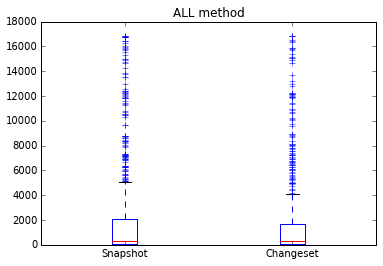
\includegraphics[width=0.4\textwidth]{figures/all_method}
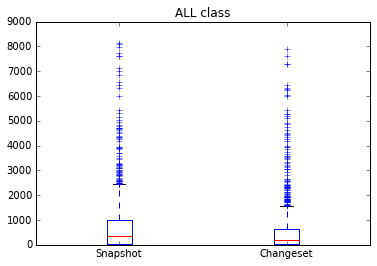
\includegraphics[width=0.4\textwidth]{figures/all_class}
\caption{Effectiveness measures for methods and classes across all systems}
\label{fig:em}
\end{figure*}

Figure~\ref{fig:em} shows the effectiveness measures for methods and classes
across all systems. The figure suggests that snapshot-based models and
changeset-based models have similar results overall, but does not help to
understand how each feature query performs for each model.
With respect to RQ1, we will investigate the queries and effectiveness measures in detail.

For the 1214 successful queries of classes,
each query returns the same effectiveness measure 30 out of 1214 times, or about 2.5\% of the time.
For 178 queries (14.7\%), the effectiveness measure is within 10 ranks of each other.
For 356 queries (29.3\%), the effectiveness measure is within 50 ranks of each other.
The remaining 858 queries (70.6\%) performs noticibly worse ($> 50$ ranks apart).

For the 629 successful queries of methods,
each query returns the same effectiveness measure 12 out of 629 times, or about 1.9\% of the time.
For 65 queries (10.3\%), the effectiveness measure is within 10 ranks of each other.
For 151 queries (24.0\%), the effectiveness measure is within 50 ranks of each other.
The remaining 478 queries (76.0\%) performs noticibly worse ($> 50$ ranks apart).


\begin{table}[t]
\renewcommand{\arraystretch}{1.3}
\footnotesize
\centering
\caption{ArgoUML v0.26.2 Queries}
\begin{tabular}{r|p{0.8\linewidth}}
\toprule
Feature \# & Bag-of-words representation  \\
\midrule
5088       &

profiles (4),
xmi (3),
user (3),
profile (3),
write (3),
save (2),
files (2),
defined (2),
loaded (2),
impl (2),
mdr (2),
writer (2),
models (2),
able (1),
available (1),
implemented (1),
file (1),
model (1),
issue (1),
release (1),
aren (1),
using (1),
isn (1),
zargo (1),
creating (1),
removed (1),
configuration (1),
removing (1),
empty (1),
won (1),
seams (1),
persister (1),
usage (1),
simply (1),
written (1),
depend (1),
due (1),
configured (1),
deeper (1),
directories (1),
experimentally (1),
flag (1),
functionality (1),
persist (1),
prevents (1),
tackle (1),
unassigned (1),
wasn (1),
writing (1)

\\
5258       &

name (2),
classifier (2),
perspective (2),
collaboration (2),
rules (2),
explorer (1)

\\
\bottomrule
\end{tabular}
\label{table:argoumlqueries}
\end{table}



ArgoUML v0.26.2 feature 5258 has an effectiveness measure of 1 under the
snapshot-based model and 8138 under the changeset-based model, while feature
5088 had 1 under the changeset-based model and 124 under the snapshot-based
model.  Table~\ref{table:argoumlqueries} shows the bag-of-words representation
of each feature query.

Feature 5258 returns 3 related snapshot topics: 194 (58\%), 226 (18\%), and 464 (14\%).
The most related snapshots topics of the first relevant method at rank 1,
\texttt{GoClassifierToInstance.getRuleName()},
are also 194 (82\%), 226 (6\%), and 464 (4\%).
Hence, the snapshot model performs as expected.
Feature 5258 returns 2 related changeset topics: 250 (48\%) and 365 (43\%).
Unforunately, the first relevant method at rank 8138,
\texttt{GoClassifierToInstance.getRuleName()},
returns 2 different changeset topics: 432 (76\%) and 332 (17\%).
However, with the exception of changeset topic 432, the top words in these
topics are similar to that of the query. Changeset topic 432 appears to be a general
topic, consisting of words like ``jar'' (8\%), ``argouml'' (6\%), and ``org'' (5\%).

Feature 5088 returns 18 snapshot topics, with 3 highly ($> 10\%$) related: 281 (19\%), 283 (13\%), and 38 (11\%).
There are 6 snapshot topics for the first relevant method at rank 142,
\texttt{XmiWriterMDRImpl.write()},
and the highly related topics are 283 (56\%), 82 (16\%), and 41 (12\%).
We note that both each of these contain snapshot topic 283,
but the feature does not relate as highly to the topic as the method does.
We also note that the model seems confused about which topics are related to the feature.
Feature 5088 returns 19 changeset topics, with 3 highly related: 446 (21\%), 426 (12\%), and 472 (11\%).
The first relevant method at rank 1,
\texttt{testWritePreviouslyLoadedProfile()},
returns 10 changeset topics, with 3 highly related: 446 (47\%), 462 (15\%), and 426 (12\%).
7 out of the 10 changeset topics also appear in the 19 related to the feature.
Here, the changeset model was able to better discern which topics were related to the feature.


\begin{comment}


\begin{table}[h]
\renewcommand{\arraystretch}{1.3}
\footnotesize
\centering
\caption{MuCommander v0.8.5 Queries}
\begin{tabular}{r|p{0.8\linewidth}}
\toprule
Feature \# & Bag-of-words representation \\
\midrule
37         &

        mac (3),
        menu (3),
        window (2),
        minimize (2),
        missing (2),
        zoom (2),
        application (1),
        mimic (1),
        options (1),
        standard (1)


\\
142       &

        java (7),
        drive (6),
        icons (3),
        button (3),
        popup (3),
        names (3),
        refresh (3),
        exception (2),
        hashtable (2),
        main (1),
        lang (1),
        mucommander (1),
        com (1),
        util (1),
        npe (1),
        pointer (1),
        run (1),
        thread (1),

\\
\bottomrule
\end{tabular}
\label{table:muqueries}
\end{table}



MuCommander v0.8.5 feature 37 has an effectiveness measure of 1 under the
snapshot-based model and 303 under the changeset-based model, while feature 142
had 1 under the changeset-based model and 536 under the snapshot-based model.
Table~\ref{table:muqueries} shows the bag-of-words representation of each
feature query.

\end{comment}

%%%% Awkwardddddddddd

In this study, we've also asked two research questions which lead to two
distinct comparisons.  First, we compare a batch topic-modeling-based FLT
trained on the changesets of a project's history to one trained on the snapshot
of source code entities.  Second, we compare a batch topic-modeling-based FLT
trained on changesets to a online topic-modeling-based FLT trained on the same
changesets over time.  With respect to RQ2, our results are mixed, hence we end
up with four possible situations; we will now discuss each of these situations
in detail.

%
% Old blah-de-blah.
%
\subsubsection{Batch changesets are better than batch shapshot
\emph{and} batch changesets are better than changesets in the simulated environment}

% Snapshots < Changeset && Batch > Temporal
% Class
%   ArgoUML 0.24
%
% Method
%   ArgoUML 0.22

This situation occurs in
1 out of 6 systems at the class-level, and
1 out of 6 systems at the method-level.
We hypothesize that this is due to the nature of the batch evaluation versus the historical simulation.
In the batch evaluation, the model is trained on all data before being queried,
while in the historical simulation the model is trained on partial data before being queried.
This allows for the batch model to be more accurate because it is trained on more data
and reveals feature location research evaluations may not be accurately portraying
how an FLT would perform in a real scenario.

\subsubsection{Batch changesets are better than batch shapshot
\emph{and} changesets in the simulated environment are better than batch changesets}

% Snapshots < Changeset && Batch < Temporal
% Class
%   ArgoUML 0.22
%
% Method
%   JabRef
%   jEdit
%   muCommander

This situation occurs in
1 out of 6 systems at the class-level, and
3 out of 6 systems at the method-level.
We hypothesize that this is due to the same previous reason, but that
historical simulation more accurately captures the correct state of the system (i.e., the source code entities)
at the point in time when querying is done.
Since querying on the batch models is after the model is completely trained,
there may be source code entities that do not exist in the system anymore
that were at one time changed to complete a certain task.
Again, the historical simulation better captures this scenario.

\subsubsection{Batch snapshot are better than batch changeset
\emph{and} changesets in the simulated environment are better than batch changesets}

%  Snapshots > Changeset && Batch < Temporal
% Class
%   ArgoUML 0.26
%   JabRef
%   jEdit
%   muCommander
%
% Method
%   ArgoUML 0.24
%   ArgoUML 0.26

This situation occurs in
4 out of 6 systems at the class-level, and
2 out of 6 systems at the method-level.
Similarly, this could be because of how the models are trained.
Although the batch changesets performed worse in both cases, it does
improve during historical simulation.
This does not mean that changesets are bad, but more accurately model
the system over time.

\subsubsection{Batch snapshot are better than batch changeset
\emph{and} batch changesets are better than changesets in the simulated environment}

% Snapshots > Changeset && Batch > Temporal
% Class
%
% Method
%
We note that this situation never occurs.
This also supports the hypothesis that historical simulation more accurately portrays the system over time.
However, we cannot conclude this without also historically simulating snapshot-based topic models.
